\chapter{Teori}
\label{cha:theory}
Det här kapitlet ämnar redogöra för de verktyg och begrepp som är viktiga att känna till för att förstå projektets innebörd.

\section{Verktyg}
\subsection{Git}
\label{sec:theory-git}
Git är en mjukvara för att versionshantera kod. Användaren kopplar sig via ett klientprogram till versionshanteringsarkivet via internet som ligger uppe på värdens server. 
Genom klientprogrammet kan användaren ladda upp ny kod till arkivet och hämta hem andras kod. 
Git möjliggör för flera personer att sitta och ändra i samma kod på olika ställen, för att senare kunna sammanfoga alla ändringarna på ett lätt sätt. 
Alla ändringar som görs sparas som historik så att man alltid kan gå tillbaka till äldre versioner och exempelvis se vem som gjort vad. \cite{website:git}

\subsection{Trello}
\label{sec:theory-trello}
Trello är en webbapplikation för planering där man kan skapa visuella tavlor och dela dessa med andra personer i samma projekt. 
På dessa tavlor kan man skapa och placera Trello-kort som kan flyttas runt i olika listor. 
Detta kan jämföras med en anslagstavla i den verkliga världen, där Trello-korten är post it-lappar som kan flyttas runt. 
På Trello-kort kan det skrivas kommentarer och därav föras en konversation. \cite{website:trello}

\subsection{Slack}
\label{sec:theory-slack}
Slack är en chattbaserad kommunikationsplattform som finns både för mobil och dator. 
Den är mer komplex än andra chattapplikationer då man har möjlighet att skapa kanaler och lägga till funktionalitet från tredje part. \cite{website:slack} 

\subsection{InVision}
\label{sec:invision}
InVision är en webbaserad tjänst för att skapa digitala prototyper. 
Användaren kan ladda upp bilder och skisser av olika slag, och skapa interaktiva prototyper av skisserna. 
Detta görs genom att placera ut aktiva områden ovanpå skisserna, och ställa in vilken bild som ska visas när det aktiva området aktiveras genom klick eller att muspekaren placeras ovanpå.\cite{website:invision}

\section{Kontinuerlig integration}
Kontinuerlig integration är processen att integrera mjukvaruartefakter  kontinuerligt,
så ofta som möjligt och på så sätt i så små bitar som möjligt.
Metoden utvecklades för att undvika det så kallade "integrationshelvetet" som
vanligtvis uppstår då man skjutit upp integrationen till den punkten att det är en verklig utmaning att
sammanfoga alla komponenter och få dem att fungera tillsammans. \cite{continous_integration}

\begin{figure}[h]
  \centering
  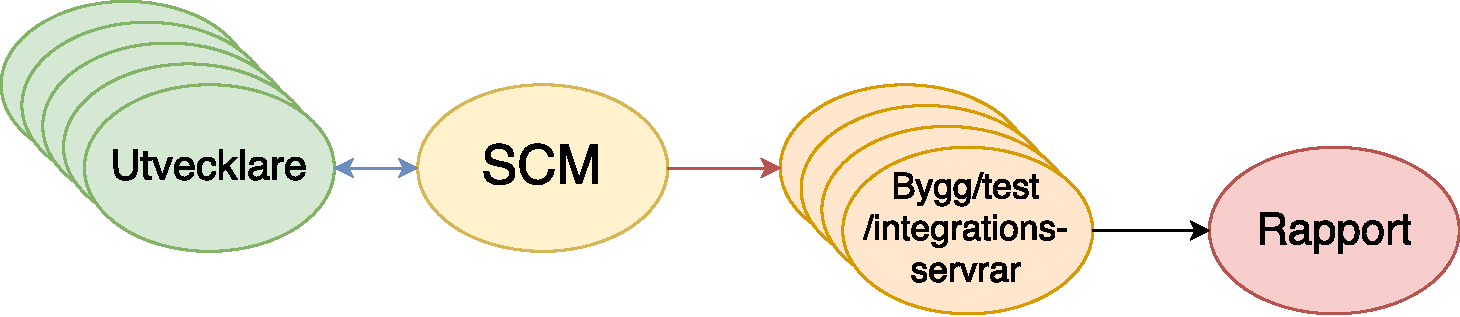
\includegraphics[scale=0.4]{ci_workflow}
  \caption{En illustration över ett KI-flöde.}
  \label{fig:ci_workflow}
\end{figure}
\ \\
För att kunna integrera artefakter så ofta som flera gånger per dag behövs en automatiserad process
som säkerställer de integrerade artefakternas kvalitet. En illustration över hur det skulle kunna se ut ses i figur \ref{fig:ci_workflow},
där en mängd utvecklare arbetar mot en server för Software Control Management (SCM) som meddelar en mängd servrar förändringar som i sin tur automatiskt kompilerar,
testar och integrerar den nya mjukvaran för att sedan rapportera hur det gått.

\section{Scrum}
\label{sec:scrum}
Scrum är ett ramverk för agila utvecklingsmetoder som utvecklades under 1990-talet, med värdeorden
transparens, inspektion och anpassning.\cite{website:scrum_guide} Viktiga aspekter som det medför är 
\begin{enumerate}
\item Eftersträva transparens mot kund
\item Jämför producerade artefakter mot krav
\item Vara redo för förändringar i krav
\end{enumerate}
\ \\
För att beskriva Scrum är det rimligt att jämföra det med den traditionella
\textit{vattenfallsmodellen} .\cite{production_of_large_computer_programs}
Det är en metod som tagits från tillverkningsindustrin och tillämpats på mjukvaruindustrin och
som kritiserats för dess oförmåga att hantera förändringar i krav och projektdirektiv.
\begin{figure}[H]
  \centering
  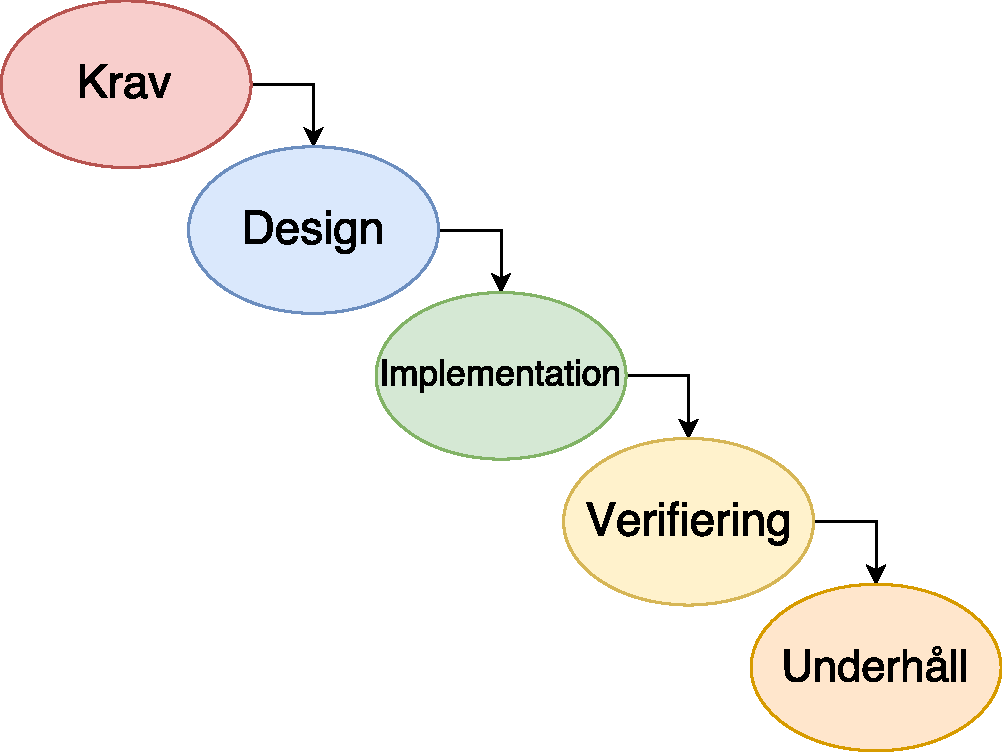
\includegraphics[scale=0.33]{waterfall_workflow}
  \caption{En illustration över vattenfallsmodellens olika stadier.}
  \label{fig:waterfall_workflow}
\end{figure}
\ \\
Ett projekt som följer vattenfallsmodellen har tydliga
faser som i följs i sekvens, från framtagning av krav till underhåll. En illustration av vattenfalls
modellen kan ses i figur \ref{fig:waterfall_workflow}.
Till skillnad från vattenfallsmodellen ristas krav ej i sten inom Scrum, och olika moment i
projektet kan itereras på. En grupp som tillämpar Scrum har en utsedd \textit{produktägare}
som ansvarar för att besluta vilka funktionalitetskrav som ger mest värde för kund och i
vilken ordning det bör utföras. Krav kan även omformuleras, tillkomma och
kasseras genom hela projektet. Produktägaren sammanställer kraven i en \textit{produkt-backlog}
som är en lista på funktionalitet sorterad på prioritet vilken representerar projektets
omfång vid ett tillfälle. Produkt-backlogen lägger grund för vad som ska utföras i utvecklingsarbetet.
\\ \\
Utvecklingen i Scrum struktureras i \textit{sprinter} på två till fyra veckor. Inför en sprint
bestämmer sig gruppen för en mängd arbete som skall utföras, plockat från produkt-backlogen
varpå den läggs i projektets \textit{sprint-backlog}. Sprint-backlogen är till skillnad från
produkt-backlogen låst och får ej ändras under sprinten. Detta för att ge
gruppen möjlighet att fokusera på och organisera sig kring en konstant mängd arbete.
\\ \\
Under en sprint hålls dagliga möten som får ta max en kvart där alla gruppmedlemmar
närvarar och svarar på frågorna
\begin{enumerate}
\item Vad har du gjort sen senast?
\item Vad ska du göra idag?
\item Vilka problem förutspår du?
\end{enumerate}
\ \\
Scrum-mötena ökar transparensen bland de deltagande och ger möjligheten att bemöta hinder
innan de uppstår. Det är gruppens utsedda \textit{Scrum master} som ansvarar för
att organisera mötena, och denna arbetar också för att underlätta utvecklingsarbetet.
Efter varje sprint utvärderar gruppen sprinten och förbättringsförslag till kommande sprinter tas fram.
Produktägaren presenterar även arbetet som sprinten resulterade i för kund och omarbetar krav baserat
på kundens åsikter.

\section{Kanban}
\label{sec:kanban}
Kanban är en arbetsmetodik som går ut på att en grupp har en tavla med kort som från början placeras i en produkt-backlog. 
\cite{website:atlassian_kanban} Korten med uppgifter flyttas sedan genom arbetsflödet allt eftersom uppgifterna färdigställs. 
Ett typiskt arbetsflöde innehåller en produkt-backlog, pågående uppgifter, färdiga uppgifter som behöver granskas och klara uppgifter. Nya uppgifter läggs till vid behov och ingen uppgift har en specifik tidsbudget.

\begin{figure}[H]
  \centering
  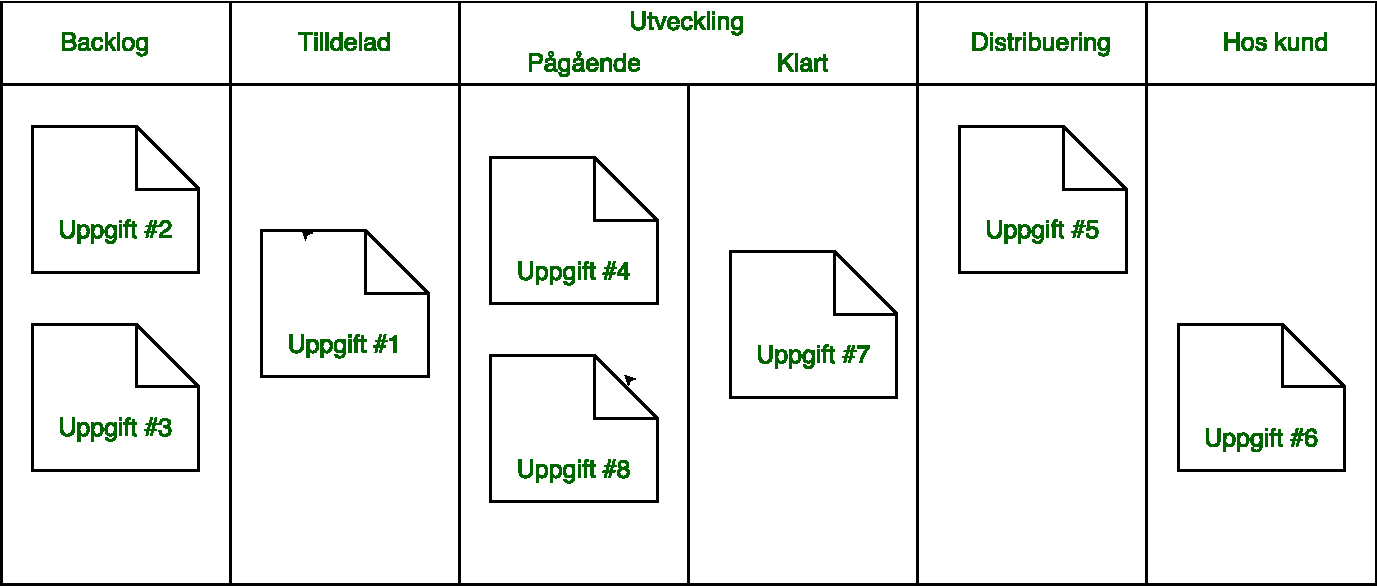
\includegraphics[scale=0.4]{Kanban_v2}
  \caption{En illustration över Kanbans flödesschema.}
  \label{fig:kanban_workflow}
\end{figure}
\ \\
I figur \ref{fig:kanban_workflow} visas ett typiskt arbetsflöde inom Kanban. Gruppmedlemmarna får själva plocka uppgifter från produkt-backlogen för att sedan utföra dem.

\section{Feature branch-arbetsflöde}
\label{sec:feature-branch-workflow}
\textit{feature-branch-arbetsflödet} går ut på att isolera stabil funktionalitet från
funktionalitet som är ny eller under utveckling genom att använda Gits funktionalitet
\textit{grenar}.\cite{website:atlassian_git}
Det finns alltid en stabil gren som kallas för \textit{mästergrenen} och en gren med ny
funktionalitet som kallas för \textit{utvecklingsgrenen}. När ny funktionalitet ska utvecklas
görs en förgrening från utvecklings-grenen till en \textit{funktionalitetsgren} där all
utveckling sker. När funktionaliteten är klar sammanfogas funktionalitetsgrenen med
utvecklingsgrenen igen, som sedan kan testas noggrant innan den i sin tur
sammanfogas med mästergrenen. På så sätt är alltid mästergrenen i leveransbart tillstånd.

\section{Informationsvisualisering}
\label{sec:info-vis}
Att visa data med flertalet attribut kan göras på många olika sätt. Något av det mest simpla sätten är att visa data i en tabell, där varje objekt representeras av en rad, och för varje attribut finns en kolumn. 
De flesta känner sig hemma med att hantera en tabell, men det kan vara begränsande för användaren att hitta den data som eftersöks i tabell. Speciellt svårt blir det när det finns många rader och tio eller fler kolumner. 
Även om önskad data hittas, så kan användaren fortfarande ställa sig frågan vad mer som gömmer sig i datamängden. Finns det liknande alternativ? Finns det oupptäckta mönster eller korrelationer?
En lösning till detta kan vara att lägga in möjligheten att sortera tabellen baserat på de olika attributen, och på så sätt få en interaktiv omplacering.
Andra lösningar kan vara att presentera datan på ett helt annrolunda sätt, för att på så sätt förändra användarens mentala modell av hur datamängden ser ut. Om den mentala modellen ser annorlunda ut, ger detta användaren en möjlighet att se datan på ett annat sätt och göra upptäckter som inte hade gjorts i en tabell. \cite{information-visualization}. % ok

\section{Prototyper}
\label{sec:prototypes-theory}
En prototyp inom utveckling av användargränssnitt till mjukvara är en version av det slutgiltiga systemet eller delar av det, med begränsad eller ingen funktionalitet. Målsättningen med prototyper är att i ett tidigt skede i utvecklingen hitta lösningar och designer av systemet för att användaren ska kunna ha så stor nytta av systemet som möjligt. \cite{arvolaboken} För ett system där större delen av funktionaliteten baseras på användarens interaktion och tolkning av gränssnittet kan också funktioner utvecklas inom ramarna för prototyparbetet.
\\ \\
Det finns många olika sorters prototyper. De kan göras på papper, digitala skisser, delvis kodade eller helt baserat på kod. De kan ha olika grad av interaktion och de styrs eller hanteras på olika sätt.
De olika typerna har olika fördelar och passar i olika delar av ett projekt beroende på vilken information man vill få ut från dem. Pappersprototyper lämpar sig allra bäst i början av ett projekt då man vill få de mest övergripande idéerna, men kan också fungera i slutet på ett projekt när mer detaljerade designbeslut ska tas.
\\ \\
En risk med prototyper är att de kan vara \textit{underpresterande} eller \textit{överpresterande}.
Underpresterande prototyper är obestämda och ambiguösa till den nivån att betraktaren har maximalt utrymme för tolkning, vilket kan vara riskabelt. Detta kan leda till att alla inte delar samma bild av vad prototypen representerar.
Överpresterande prototyper har för hög detaljeringsgrad i ett för tidigt skede i ett projekt. Detta kan upplevas som imponerande, men riskerar att medföra att designbeslut tas för tidigt i ett projekt. Detta kan i sin tur medföra att slutprodukten inte blir lika bra som den hade kunnat bli, eftersom många designalternativ uteslöts alldeles för tidigt. 
Effektiva prototyper är en bra balans mellan under- och överpresterande prototyper. De har tillräckligt mycket detaljer för att utvecklingsgruppen ska kunna tolka dem och få inspiration till nya designidéer, men också tillräckligt öppna med utrymme för inga beslut ska tas för tidigt. \cite{effective-prototyping}
\\ \\
Det finns en risk när man arbetar med agila metoder som till exempel Scrum (se avsnitt \ref{sec:scrum}) att utvecklingsteamet hoppar över det inledande konceptarbetet och kastar sig direkt på mjukvaran och börjar programmera. Detta kan leda till att teamet i slutet av projektet har en applikation som mycket möjligt kan vara väl implementerad, men som inte är genomtänkt i aspekterna helhet eller nytta för användaren. \cite{arvolaboken}

\section{Användbarhetstest}
\label{sec:usability-tests}
Användbarhetstester är tester som utförs för att få information om hur väl en användare kan förstå och använda ett system. Testerna kan utföras på prototyper, delsystem eller slutgiltigt system. Testerna är en del av utvecklingsprocessen och bör användas kontinuerligt genom ett helt projekt för att
säkerställa att systemets uppdateringar följer användarnas förmåga att använda det.\cite{effective-prototyping}

\section{635-metoden}
635-metoden är en metod för att få fram idéer. Sex personer skriver idéer på papper för att svara på en frågeställning på fem minuter. Varje person skriver tre egna idéer. När fem minuter har gått så skickas papperna vidare runt i en cirkel så att alla får skriva tre nya idéer på nästa papper. Detta återupprepas tills alla har skrivit tre idéer på alla papper. Slutligen grupperas idéerna efter relevans och likhet med varandra. \cite{arvolaboken}

\section{Mjukvara som applikationen baseras på}
\label{sec:software-base}
Här förklaras kortfattat vilken mjukvara som gruppen inte egenhändigt har tillverkat men som applikationen använder sig av. Alla dessa underliggande applikationer, ramverk eller databaser var önskade av kund att användas i utvecklingen.

\subsection{Eiffel}
\label{sec:eiffel}
Eiffel är ett ramverk för kontinuerlig integration som försöker lösa problemet att en stor
mängd enheter behöver kommunicera med varandra igenom ett KI-flöde. Det är tillämpbart på all
kommunikation som sker från och med att en kodändring kommit till SCM i figur \ref{fig:ci_workflow}.
Ramverket möjliggör att sända plattformsoberoende händelser över en gemensam kanal
och på så sätt standardisera kommunikationen mellan alla servrar igenom flödet.\cite{website:eiffel}
\\ \\
Genom att samla all automatiserad kommunikation under samma protokoll möjliggör även Eiffel att samla in och spåra alla händelser i ett KI-flöde på ett enkelt sätt och det är på sådan data applikationen baserar sin rendering.

\subsection{MongoDB}
\label{subsec:mongodb}
MongoDB är en dokumentdatabas. Olikt en relationsdatabas så lagrar MongoDB data i dokument och returnerar data som till exempel JSON-objekt. Den MongoDB-databasen som applikationen använder är inbyggd i Meteor, men om så skulle önskas så kan en MongoDB-databas delas upp på olika hårdvara för att sprida ut arbetsbelastningen. \cite{website:mongodb}

\subsection{Node.js}
\label{subsec:node}
Node.js är en exekveringsmiljö för JavaScript baserat på öppen källkod som ofta används för att köra serverapplikationer. Många av basmodulerna och funktionerna i Node.js är skrivna i JavaScript, men även i C och C++. Node.js tolkar JavaScript med hjälp av Googles JavaScriptmotor V8 och har stöd för asynkrona funktionsanrop. På så sätt kan flera anrop behandlas parallellt när det körs på en server. \cite{website:nodejs}

\subsection{Meteor}
\label{subsec:meteor}
Meteor är ett ramverk för webbutveckling i JavaScript baserat på öppen källkod. Ramverket är byggt på Node.js, se avsnitt \ref{subsec:node}, och möjliggör implementation av både front-end och back-end i JavaScript. Meteor möjliggör snabb prototypning, integrerar med MongoDB och distribuerar dataändringar automatiskt till klienter utan att utvecklaren behöver skriva kod för synkronisering. \cite{website:meteor}

\begin{figure}[h]
  \centering
  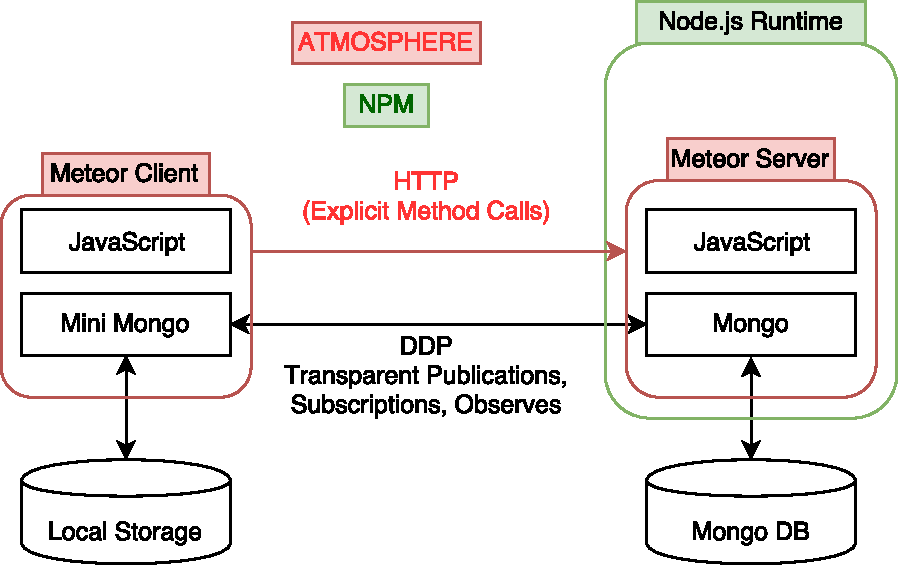
\includegraphics[scale=0.4]{Meteorarchitecture}
  \caption{En illustration över Meteors arkitektur.}
  \label{fig:meteorarchitecture}
\end{figure}
\ \\
Figur \ref{fig:meteorarchitecture} visar hur de andra mjukvarukomponenterna som Meteor använder sig av länkas samman. \textit{NPM} som visas i figuren är pakethanteraren för Node.js.\cite{website:npm} \textit{ATMOSPHERE} är katalogen för Meteor-paket.
\\ \\
Meteor tillför många kvaliteter till applikationen. Vid utveckling av en Meteor-applikation så behövs
t.ex. bara ett språk, JavaScript. Meteor har även väldigt många smarta paket att
tillgripa som sparar en mängd tid och fler paket är ständigt inom utveckling. \cite{website:atmosphere}

\subsection{HTML}
\label{sec:html}
HTML är en förkortning för \textit{HyperText Markup Language} och är ett märkspråk för hypertext. HTML är ett av språken som en webbsida kan skrivas i och hade sitt genombrott under 1980-talet då datorer kommersialiserades för hushållen. 

\subsection{CSS}
\label{sec:css}
CSS är en förkortning för \textit{Cascading Style Sheets} och är ett språk som beskriver presentationsstilen för ett dokument, såsom färg, typsnitt och textstorlek. CSS är ett språk man använder för att designa innehåll på webbsidor.


\subsection{Bootstrap}
Gränssnittsramverket Bootstrap 3.0 är ett väletablerat ramverk för gränssnitt på webbsidor. Ramverket bygger på öppen källkod och utvecklades av företaget Twitter. Bootstrap stödjer också responsiva gränssnittskomponenter för utveckling av applikationer på mindre, handhållna enheter.\cite{website:bootstrap}
